\chapter{Estado del arte}

En este capítulo se introducirán varios de los conceptos clave que se mencionarán a lo largo del trabajo, definiéndolos y detallando su estado actual respecto al ámbito de este proyecto. Con esto se facilitará el entendimiento de todo aquello que se explique en los capítulos posteriores.

El capítulo se compone de dos partes diferenciadas. Primero, se describirán distintos aspectos y tecnologías relativos al dominio del problema como el estándar actual de las aplicaciones de realidad virtual, las operaciones booleanas y las colisiones en entornos 3D interactuables y su coste computacional. Después, se analizarán otros trabajos que tengan el objetivo final de esculpir en realidad virtual, además de proyectos que, aunque no tengan el mismo objetivo, usen las mismas herramientas que esta aplicación.

\section{Dominio del problema}

Aquí se discutirán los conceptos más importantes en relación al dominio del problema para poder entender posteriormente el resto del trabajo: estado actual de las aplicaciones en realidad virtual, estándares de calidad y salud; y las operaciones booleanas, sus usos y las opciones que nos ofrece al combinarlas con hardware y software modernos, además del conflicto que suponen al usarlo en tiempo real con simulación de colisiones.

\subsection{Aplicaciones de Realidad Virtual}

En el capítulo 1 ya se ha explicado qué es la realidad virtual, pero para reiterar, es el campo de la informática gráfica que estudia la presentación e interacción con el usuario de tal forma que este se sienta trasladado a, como el nombre indica, otra realidad.

Para conseguir esto, las aplicaciones de realidad virtual deben cumplir una serie de estándares que cumplen, principalmente, dos funciones: mantener la \textbf{inmersión} del usuario y evitar el malestar físico y el peligro (\textbf{seguridad})\cite{vrstandard}. Estos estándares, debido a lo reciente que es el campo de estudio al que pertenecen, han ido cambiando considerablemente, pero se han ido asentando en años recientes. Se ahondará en las funciones mencionadas a continuación.

Primero, la inmersión. Como es de esperar, en un campo como la realidad virtual una de las principales preocupaciones es conseguir que el usuario, dentro de lo seguro y posible, se sienta dentro de la aplicación. Para conseguir esto, se deben seguir una serie de pautas. Primero, cualquier tipo de interacción con la aplicación debe ser, en la medida de lo posible, \textbf{intuitiva}. Esto conlleva usar esquemas de control que reflejen el comportamiento real de lo que se va a hacer. Un ejemplo de esto sería, al usar una pistola, que el botón de disparar fuese el gatillo del mando y no cualquier otro, o traído al ámbito de este proyecto, que un cincel y un martillo no usen en ningún momento control por botones y que únicamente sea necesario moverlos como se haría en la vida real para que funcionen. Otros elementos necesarios para una correcta inmersión es el uso de \textbf{efectos visuales y sonoros y feedback háptico} que vendan de forma correcta la acción que se está realizando. Usando los mismos ejemplos de antes, una pistola tiene que hacer un sonido concreto que lo distinga de otras armas de fuego, y un martillo golpeando un cincel producirá un sonido y una vibración mayor o menos dependiendo de la fuerza con la que se golpee.

Respecto a la seguridad y bienestar del usuario, muchas veces entra en conflicto con la inmersión. Un buen ejemplo de esto es el sistema de locomoción: aunque un movimiento libre usando el \textit{joystick} resulte más interesante y atractivo, en realidad lo más recomendado es usar un sistema de \textbf{teletransportes} a través del cual el usuario puede apuntar a una localización y desplazarse automáticamente a esta. Esto se debe a que, parecido a la sensación que puede dar ir por un terreno accidentado en un vehículo, la locomoción continua es causante de náuseas y mareos. Por esta razón, con los años se ha ido adoptando más el permitir al usuario elegir entre un sistema de locomoción y otro, generalmente estableciendo el método por teletransportes como el predeterminado (Figura \ref{fig:plantillaunreal}).

\begin{figure}[H]
	\centering
	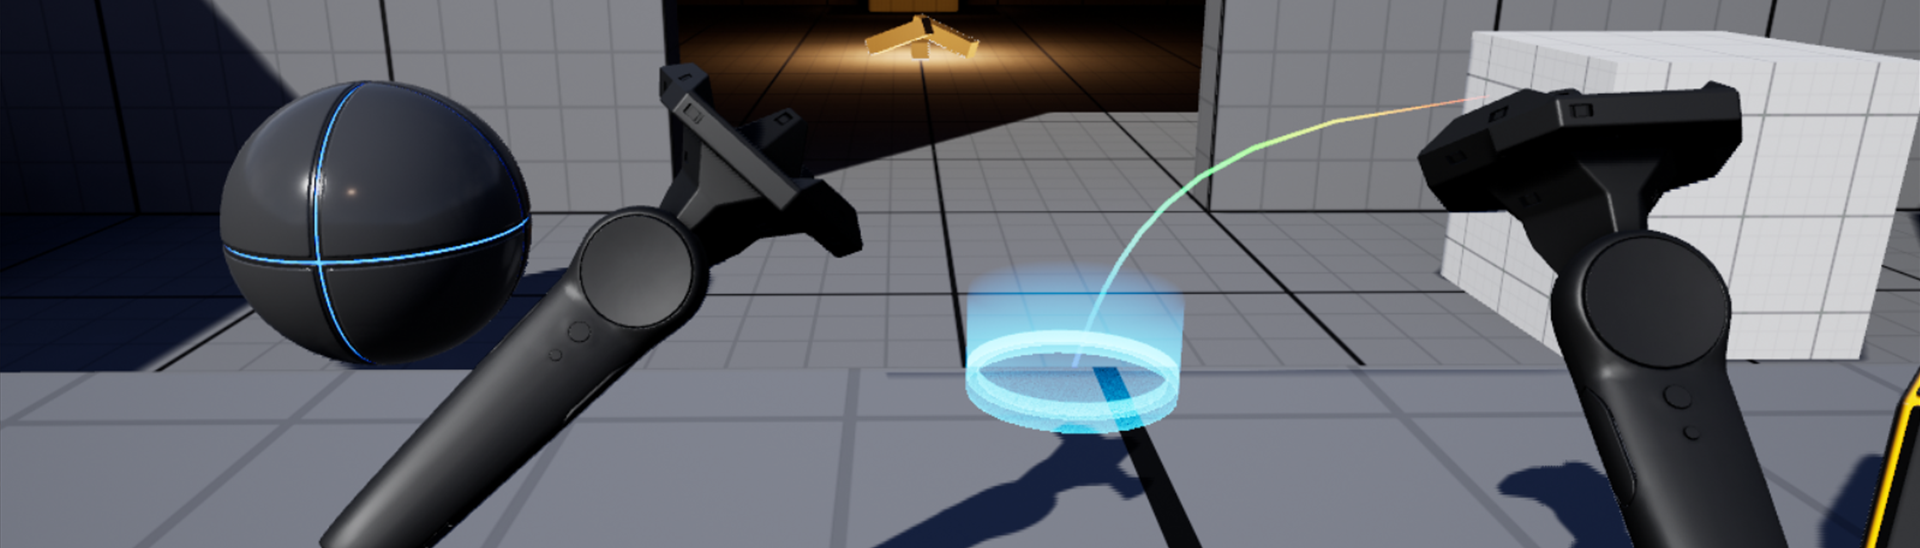
\includegraphics[width=10cm]{imagenes/plantillaunreal}
	\caption{Imagen extraída de la documentación oficial de la plantilla de proyecto VR de Unreal Engine. Se puede observar la locomoción por teletransporte siendo usada}
	\label{fig:plantillaunreal}
\end{figure}

Otro elemento importante a tener en cuenta al desarrollar con el bienestar del usuario en mente es el rendimiento de la aplicación, como ya se ha mencionado previamente. Generalmente, el ojo humano es capaz de distinguir cambios de luz y movimiento aproximadamente 60 veces por segundo, razón por la que se ha usado como estándar en muchas industrias a lo largo del tiempo. Sin embargo, esta capacidad no es estática, ya que el ojo está preparado para captar \textbf{frecuencias mucho más altas} en momentos puntuales, como cuando se perciben movimientos rápidos o se presta mucha atención en una acción \cite{refresh_rate}. En pantallas convencionales, una tasa de refresco de 60 fotogramas por segundo es más que suficiente, pero en realidad virtual es necesario alcanzar una tasa cuanto más alta mejor, pues al privar a la visión de la fluidez que percibe en el mundo real, puede llegar a causar en el usuario molestias como las mencionadas en el problema de la locomoción. Para poder alcanzar estas tasas de refresco es de gran importancia, más que en otros campos de la informática gráfica, tener muy en cuenta el rendimiento y la optimización de la aplicación.

Afortunadamente, muchos motores gráficos ofrecen plantillas a los desarrolladores para facilitar la implementación y correcto seguimiento de estos estándares. En concreto, Unreal Engine, el motor que se usará en este proyecto, ofrece en su plantilla un sistema de locomoción ya implementado y documentado con la posibilidad de ser manipulado como se desee; diferentes objetos interactuables como pistolas de los cuales partir para crear herramientas que pueda usar el usuario posteriormente; y opciones para el uso de tecnologías como FSR (\textit{Fidelity Super Resolution} de AMD), que permiten \textbf{renderizar la imagen a una calidad menor sin que se note diferencia en el resultado}, de forma que se obtiene mejor rendimiento y una tasa de refresco más alta y estable.

\subsection{Operaciones booleanas en geometría}

Para comprender las operaciones booleanas en el dominio de los entornos 3D, primero es necesario comprender en qué consisten las operaciones booleanas convencionales. Las operaciones booleanas son un conjunto de operaciones lógicas fundamentales para manipular valores binarios. Estas operaciones incluyen la negación, NOT, que cambia el valor de cualquier expresión a su contrario (es decir, de verdadero a falso y viceversa); la conjunción, AND, que devuelve verdadero únicamente si todos los valores de entrada son verdaderos; y la disyunción, OR, que devuelve verdadero si cualquiera de los valores de entrada es verdadero. Aparte de estas operaciones, existen otras derivadas de ellas las cuales no son tan relevantes para el dominio de la geometría.

Ahora, al aplicar las operaciones booleanas en la geometría, el funcionamiento es el mismo solo que en lugar de valores binarios, los datos que se manipulan son \textbf{figuras poligonales}. De esta forma, partiendo de dos objetos 3D distintos, se pueden conseguir resultados como por ejemplo el area de la primera figura sin la de la segunda, una suma de las dos o la intersección entre ambas (Figura \ref{fig:operacionesbooleanas}). En relación con las operaciones booleanas convencionales, la operación NOT se sustituye por una resta, es decir, que \textbf{la figura resultante sea la parte de la primera que \textit{no} coincide con la segunda}.

\begin{figure}[H]
	\centering
	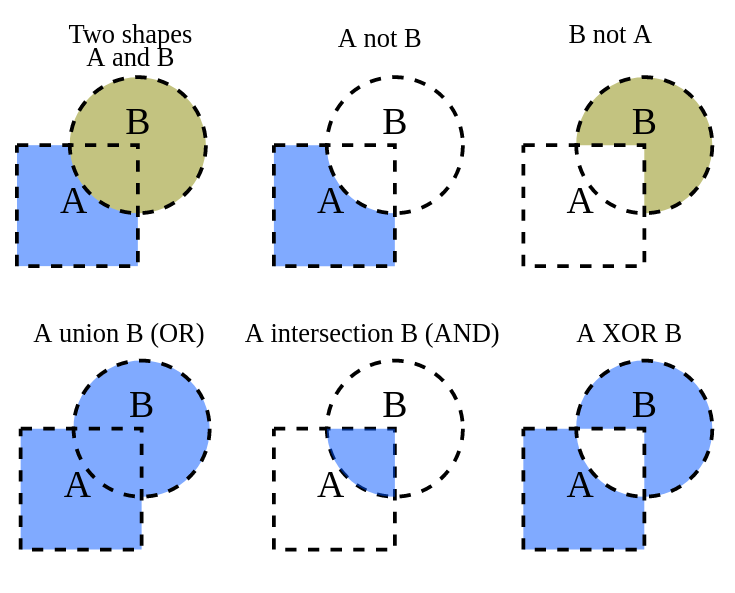
\includegraphics[width=10cm]{imagenes/operacionesbooleanas}
	\caption{Diferentes operaciones booleanas representadas en un espacio 2D}
	\label{fig:operacionesbooleanas}
\end{figure}

Incluso después de múltiples innovaciones en algoritmos para calcular las figuras resultantes de las operaciones booleanas, siguen teniendo un \textbf{alto coste computacional} y por tanto su uso siempre se ha visto reducido a aplicaciones donde el rendimiento no es de máxima prioridad \cite{boolean_operations}. Por esta razón, rara vez se ha usado en un medio interactivo como simuladores o videojuegos, menos aún en algo como realidad virtual, donde el rendimiento es clave. Pero recientemente, existen herramientas experimentales que permiten su viabilidad en este tipo de tareas.

En 2022, Epic Games lanzó un plugin experimental llamado \textbf{Geometry Script} para la última versión de su motor gráfico, Unreal Engine 5\footnote{\url{https://docs.unrealengine.com/5.0/en-US/geometry-script-users-guide/}}. Este plugin, entre otras muchas nuevas opciones de edición de generación y edición de mallas 3D, permite usar dentro de \textit{Blueprints} (equivalente en este motor gráfico a las clases en la programación por objetos) funciones normalmente solo accesibles en editores y aplicaciones de modelaje como Blender o Maya. Esto permite usar dichas funciones en tiempo de ejecución, es decir, se podrá implementar en una aplicación funcional y que el usuario final pueda usarlas para interactuar con esta. Aunque técnicamente esto era antes posible con plugins desarrollados por terceros o usando otras herramientas de gráficos 3D en base a código (como Three.js), este plugin es pionero en el uso de estas funciones de forma viable, pues hasta ahora \textbf{ninguna de estas opciones ofrecía una solución suficientemente optimizada para una aplicación de interacción en tiempo real}.

Algo relevante sobre las operaciones booleanas en el contexto de este proyecto es su relación con la simulación de colisiones. Primero, cabe destacar un dato importante sobre las colisiones: en videojuegos, simuladores y otras aplicaciones similares, \textbf{las colisiones son el factor con más coste computacional de todos}, incluso por encima de calidad gráfica y efectos visuales como las luces \cite{collisions}. Esto se debe a la necesidad de realizar una gran cantidad de comprobaciones por segundo en diferentes puntos a la vez. Por esta razón, donde más se trabaja para optimizar el coste computacional es en las colisiones, usando técnicas como la simplificación de la geometría usada para la lógica de colisiones (Figura \ref{fig:colisiones}).

\begin{figure}[H]
	\centering
	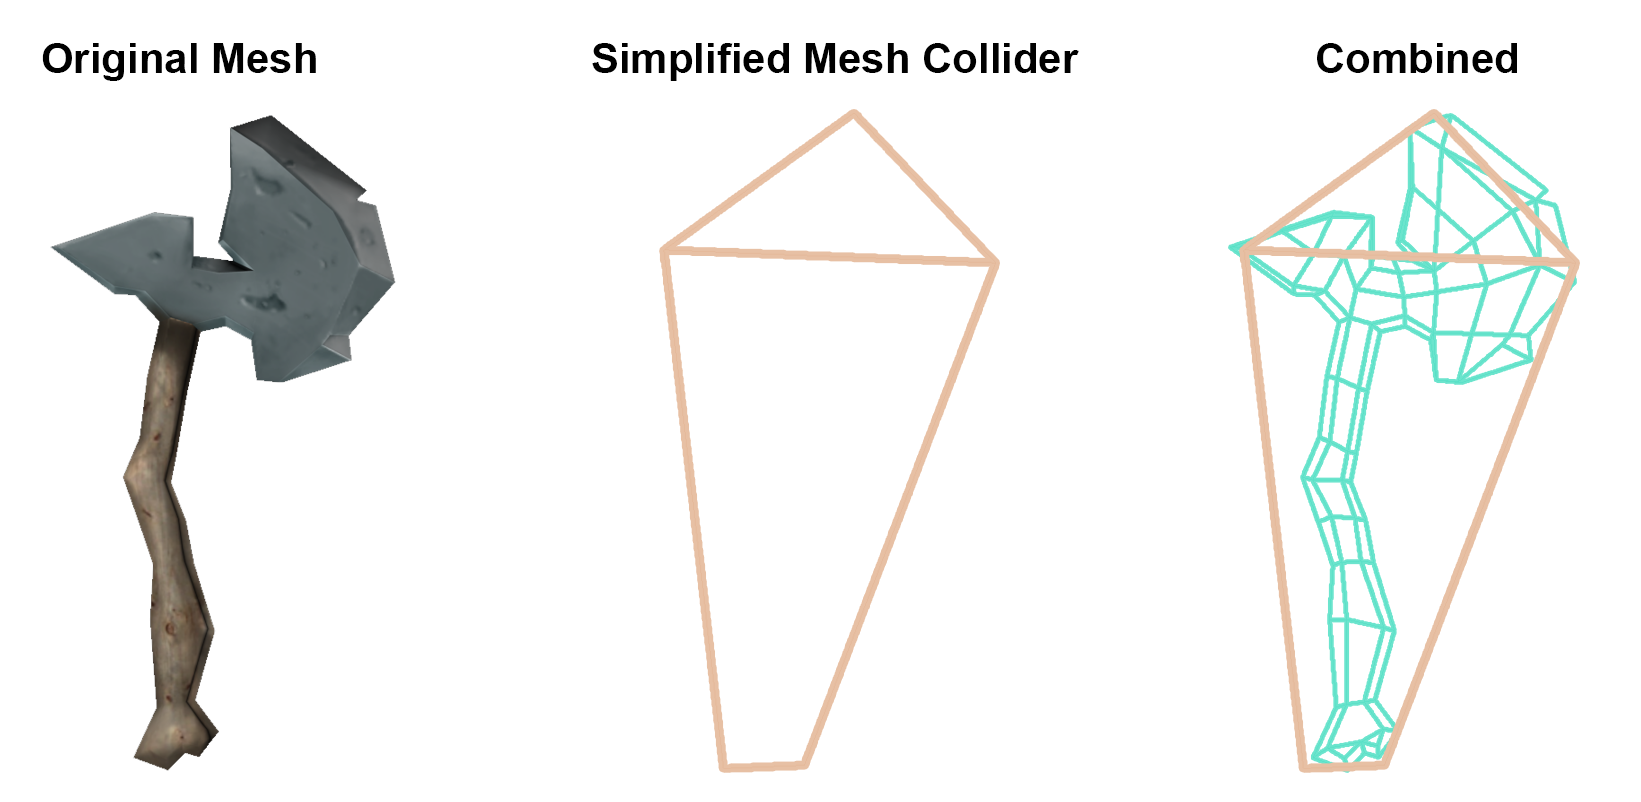
\includegraphics[width=10cm]{imagenes/colisiones}
	\caption{Comparación de la malla visual con la malla de colisión}
	\label{fig:colisiones}
\end{figure}

La razón por la que es relevante en relación a las operaciones booleanas es aparente: si se modifica la malla visual en tiempo de ejecución, también se debe modificar la malla de colisiones en caso de querer usarse en la simulación de estas. Si se deja la malla de colisiones igual que la visual, su simple existencia supone un altísimo coste computacional, mientras que si se simplifica la malla después de realizar la operación, el tiempo para realizar la operación es aún más notable, lo cual no es deseable. De hecho, en el contexto de ChiselVR, sería necesario que \textbf{ambas mallas sean iguales}, lo cual, como se ha mencionado, es algo difícil de conseguir. Por suerte, combinando el alto rendimiento de Unreal Engine 5 con hardware moderno, \textbf{ahora es algo posible}, y por tanto será lo que se usará para el desarrollo de este proyecto.

\section{Trabajos relacionados}

Aquí se discutirán otros trabajos y proyectos relacionados con la simulación de esculturas y modelaje en realidad virtual, además de otros proyectos que usan la misma tecnología que usará ChiselVR.

\subsection{Escultura en Realidad Virtual}

Como se ha mencionado en el capítulo 1, existe una gran cantidad de herramientas que permiten al usuario expresar su creatividad en realidad virtual. Entre ellas, efectivamente, existen muchas dedicadas a la creación de esculturas y otro tipo de arte tridimensional, pero con un enfoque claramente distinto al de ChiselVR: más a través de la adición de material que en la sustracción de este, y mucho más \textbf{enfocados en el resultado final} y no tanto en el arte que conlleva el proceso a este. A continuación, se profundizará en una de las aplicaciones más populares de este sector para entender mejor esta diferencia:

\subsubsection*{\textit{SculptrVR} (2016)}

SculptrVR\footnote{\url{https://www.sculptrvr.com/}} es una aplicación de modelado en realidad virtual con una gran cantidad de opciones a la disposición del usuario. Entre las herramientas más destacadas se incluyen:

\begin{itemize}
	\item Pinceles con distintos tamaños, formas y estilos para dibujar formas geométricas en el aire.
	\item Herramientas de manipulación varias, con las que modificar de diversas formas las figuras ya creadas y así realizar ajustes más precisos.
	\item Pinturas y texturas, para cambiar el aspecto de las figuras.
	\item Opciones de duplicación y simetría para facilitar la creación de este tipo de figuras.
	\item Herramientas de paisaje y escala, que permiten crear no solo objetos individuales, sino escenas completas.
	\item Funcionalidades colaborativas, con las que múltiples usuarios pueden participar al mismo tiempo en la creación de una escena.
	\item Herramientas para exportar los proyectos finalizados
\end{itemize}

Por todas las opciones listadas, su accesibilidad y su disponibilidad en múltiples plataformas, SculptrVR es de las aplicaciones más populares para la creación de objetos 3D en entornos de realidad virtual. Sin embargo, \textbf{esta aplicación no es un simulador, ni pretende serlo}: las figuras creadas flotan y no interactuan unas con otras. No bloquean el paso de las herramientas cuando estas colisionan contra su superficie, ni se parten al recibir un impacto (Figura \ref{fig:sculptvr2}).

\begin{figure}[H]
	\centering
	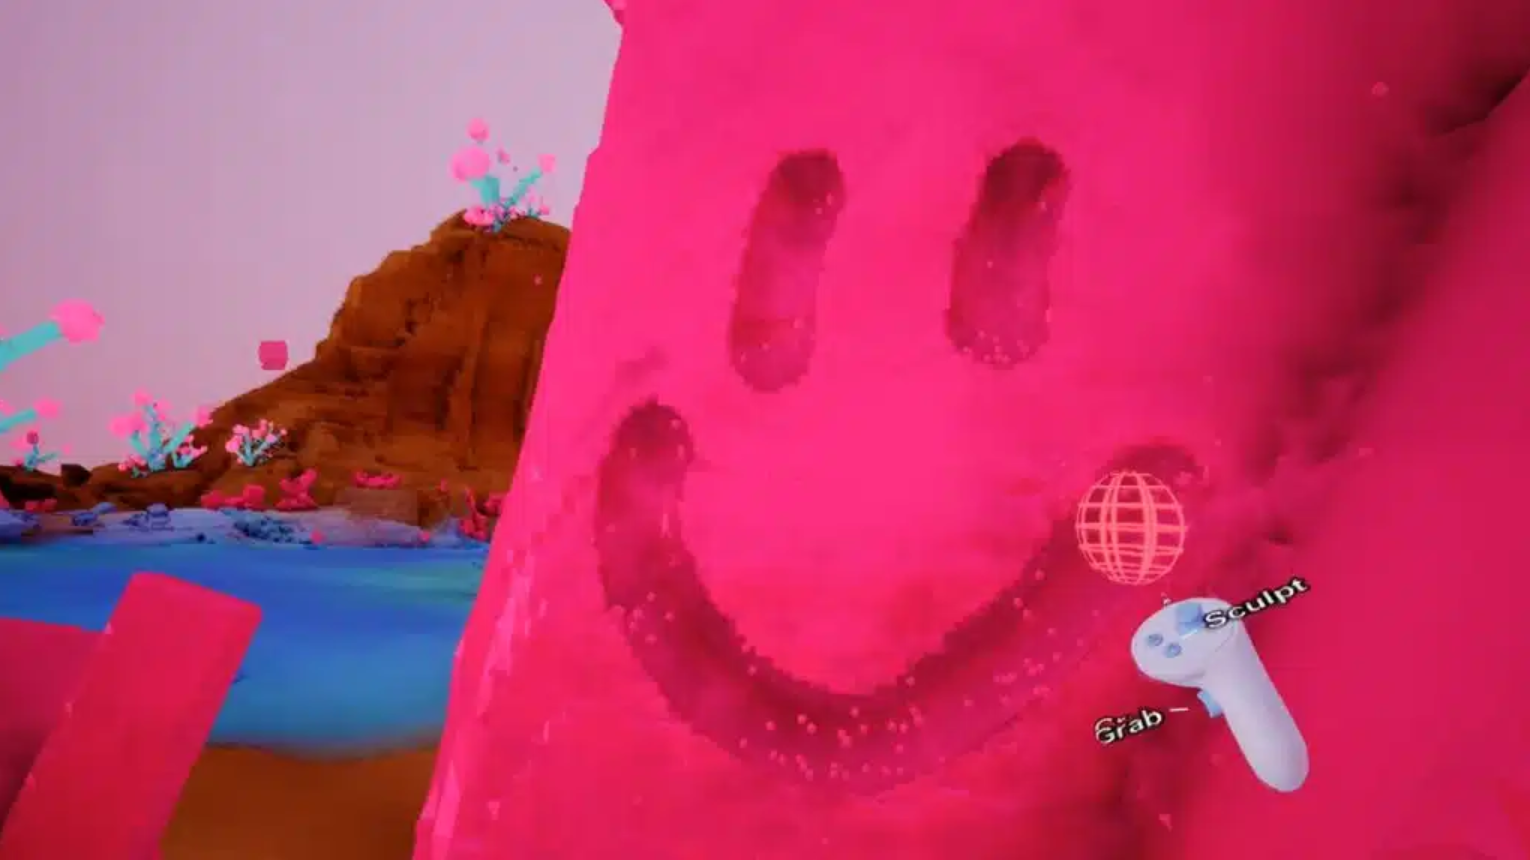
\includegraphics[width=10cm]{imagenes/sculptrvr2}
	\caption{Herramienta de tallado en SculptrVR. Aunque se elimine material de la figura, no simula la acción real de esculpido, sino que simplemente se va eliminando el material dentro del área marcada.}
	\label{fig:sculptvr2}
\end{figure}

Esto es por un lado, por supuesto, el funcionamiento deseado de la aplicación, pues su objetivo es facilitar la creatividad del usuario sin ninguna limitación, pero por otro lado es precisamente donde se distingue de este proyecto, ChiselVR, ya que el objetivo de este es simular la experiencia real de esculpir, con su dificultad y la pesada pero relajante monotonía que esta conlleva.

\subsection{Proyectos con Geometry Script}

El lanzamiento al público del plugin Geometry Script es considerablemente reciente, y aún no existen proyectos estables que lo usen. De hecho, el propio motor no lo permite, ya que Unreal Engine no tiene en cuenta elementos y funciones experimentales (como es el caso de Geometry Script) al empaquetar proyectos, es decir, crear una aplicación ejecutable sin la necesidad de usar el motor gráfico para ello.

Sin embargo, sí que existen desarrolladores trabajando en investigar las posibilidades que ofrece este plugin, y a continuación se mostrarán algunos de sus proyectos.

Primero, cabe mencionar a Ryan Schmidt, uno de los desarrolladores detrás de Geometry Script, que ha estado los últimos meses publicando tutoriales, explicaciones y experimentos usando este plugin\footnote{\url{https://www.youtube.com/@RyanSchmidtEpic/featured}}. En sus vídeos, se muestran ejemplos de uso de muchas de las funciones disponibles, tanto de forma independiente como combinándolas entre sí. Las publicaciones de este desarrollador son tan valiosas para comprender Geometry Script como la propia documentación del plugin.

Otro proyecto que muestra el potencial de Geometry Script es el experimento combinando las operaciones booleanas con proyectiles de parte del usuario de \textit{YouTube} Quantaxy\footnote{\url{https://www.youtube.com/@quantaxy}}. En este proyecto, Quantaxy usa las operaciones booleanas para crear \textbf{impactos de bala} en la pared, llegando incluso a perforar a través de esta. En resumidas cuentas, la lógica usada es:

\begin{itemize}
	\item Detectar el punto de impacto del proyectil en la pared.
	\item Calcular la velocidad del proyectil en el momento de impacto.
	\item Combinar ambos datos para calcular la profundidad del impacto en la pared.
	\item Realizar la operación booleana para eliminar material de la pared.
\end{itemize}

De esta forma, es posible crear la ilusión de que es el propio proyectil el que rompe la pared, y no a través de roturas procedurales o vóxeles (es decir, que la pared fuese compuesta por multitud de cubos pequeños en lugar de un único bloque) como se ha hecho tradicionalmente, sino con un golpe exacto y realista (Figura \ref{fig:booleans_at_runtime}). Es por eso que este proyecto, que no tiene ninguna relación con la escultura, sirvió de inspiración para ChiselVR: al esculpir, aproximaciones como en los métodos tradicionales no sirven; se necesita algo más \textbf{exacto}, y eso es exactamente lo que permite Geometry Script.

\begin{figure}[H]
	\centering
	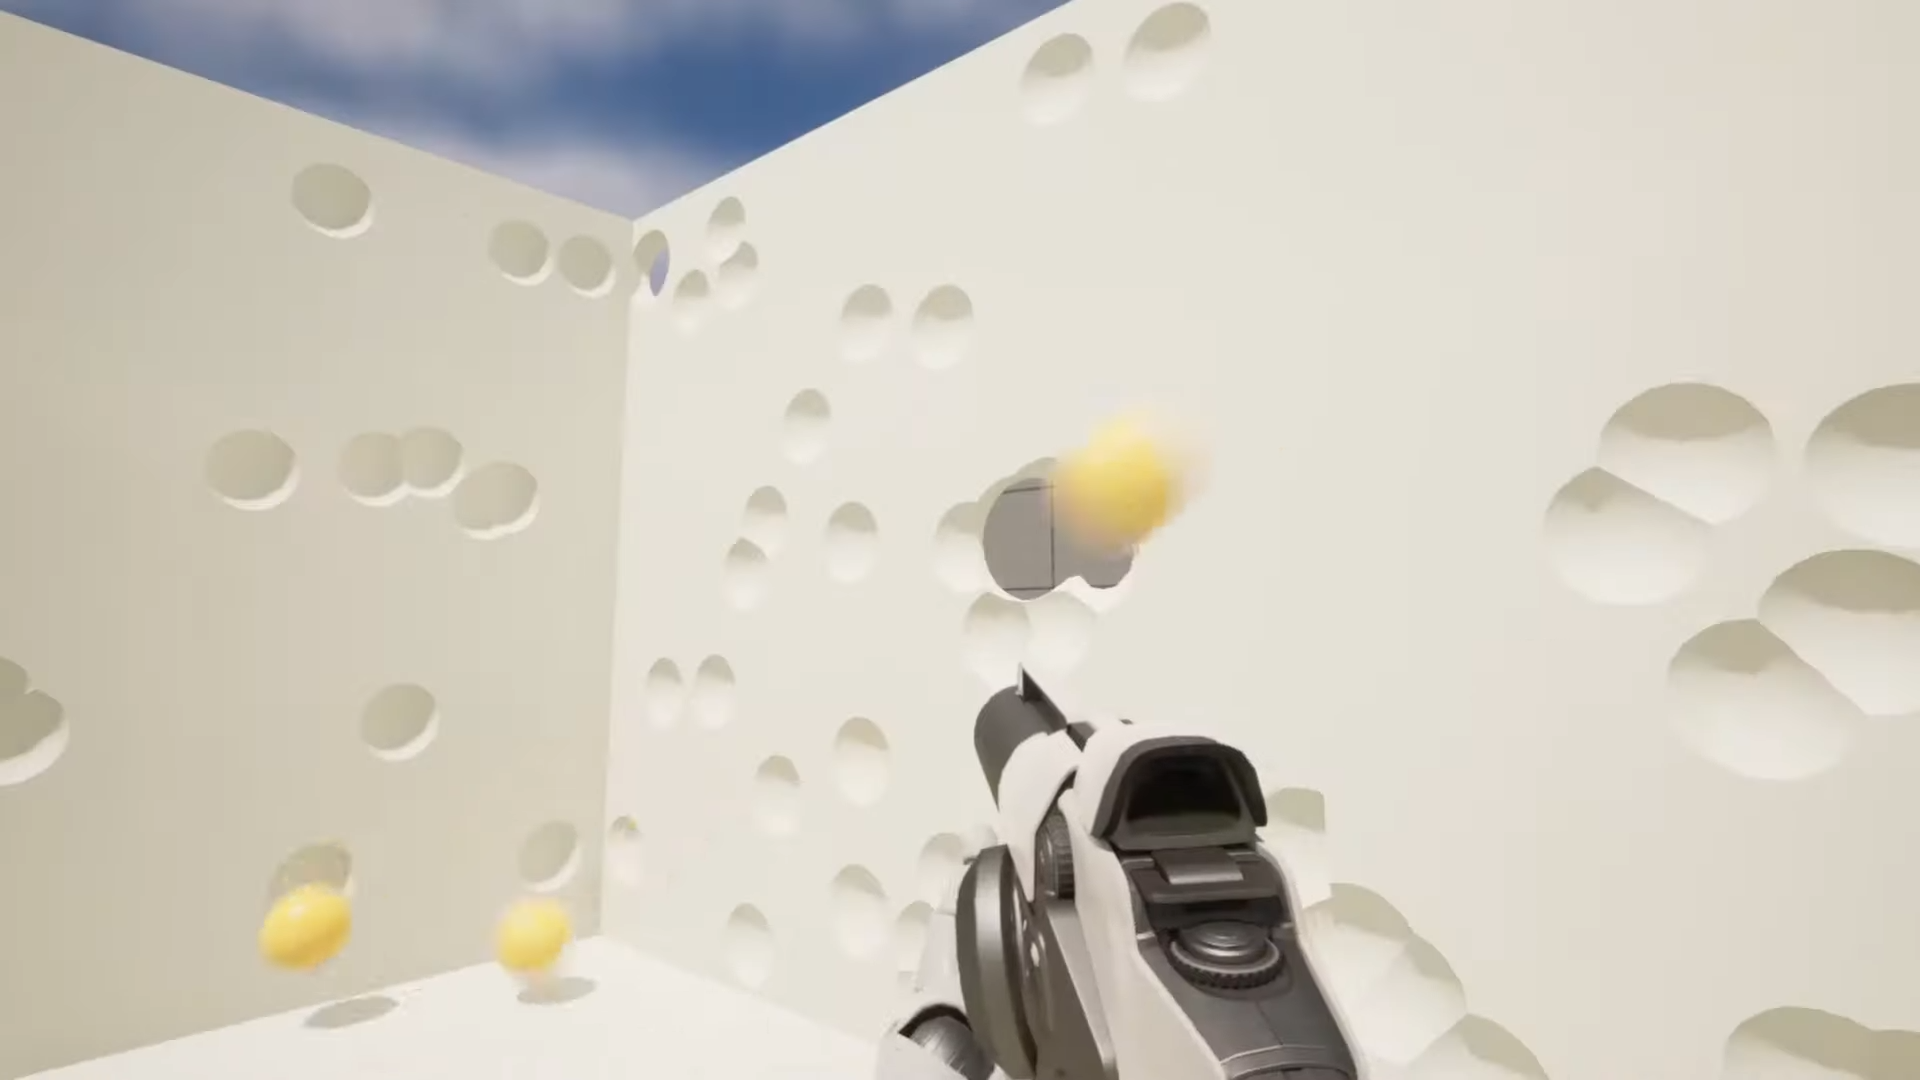
\includegraphics[width=10cm]{imagenes/booleans_at_runtime}
	\caption{Captura de pantalla del proyecto de Quantaxy en ejecución. Se pueden ver múltiples impactos en las paredes, llegando incluso a atravesar una de ellas.}
	\label{fig:booleans_at_runtime}
\end{figure}